\chapter{Конструкторская часть}

Рекуррентные формулы, рассмотренные в предыдущем разделе, позволяют находить расстояние Левенштейна и Дамерау-Левенштейна. Однако при разработке алгоритмов, решающих эти задачи, можно использовать различные подходы: итеративный алгоритм, алгоритм рекурсии с кэшированием, алгоритм рекурсии без кэширования, которые будут рассмотрены в данном разделе.

\section{Алгоритм поиска расстояния Левенштейна}

Для оптимизации нахождения расстояния Левенштейна можно использовать матрицу в целях хранения соответствующих промежуточных значений. В таком случае алгоритм представляет собой построчное заполнение матрицы. 

На рисунке \ref{fig:l_iter} приведена схема рассматриваемого алгоритма.

\begin{figure}[h!]

	\centering{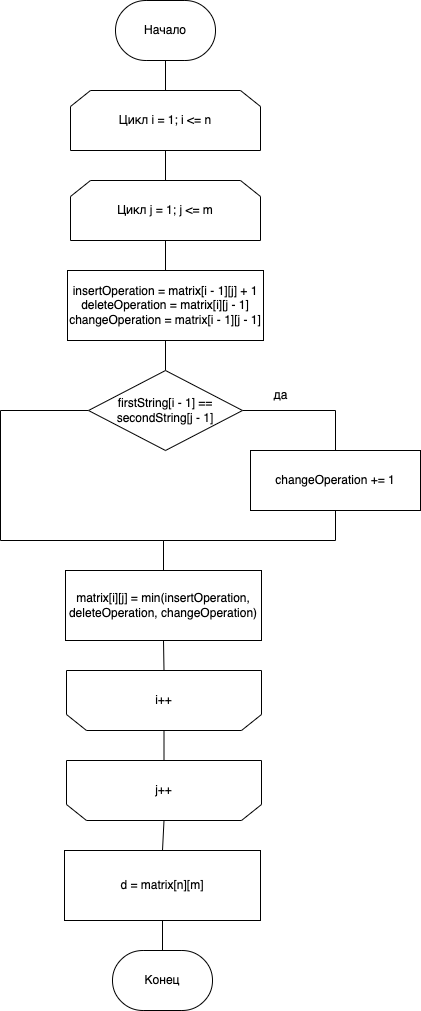
\includegraphics[scale=0.7]{img/l_iter.png}}
		
	\caption{Схема итеративного алгоритма поиска расстояния Левенштейна}
		
	\label{fig:l_iter}
\end{figure}


\section{Алгоритмы поиска расстояния Дамерау-Левенштейна}

Рассматриваются итеративный, рекурсивный без кэширования и рекурсивный с кэшированием алгоритмы поиска расстояния Дамерау-Левенштейна.

На рисунках \ref{fig:dl_iter} --  \ref{fig:dl_cash} приведены схемы рассматриваемых алгоритмов.

\begin{figure}[h!]

	\centering{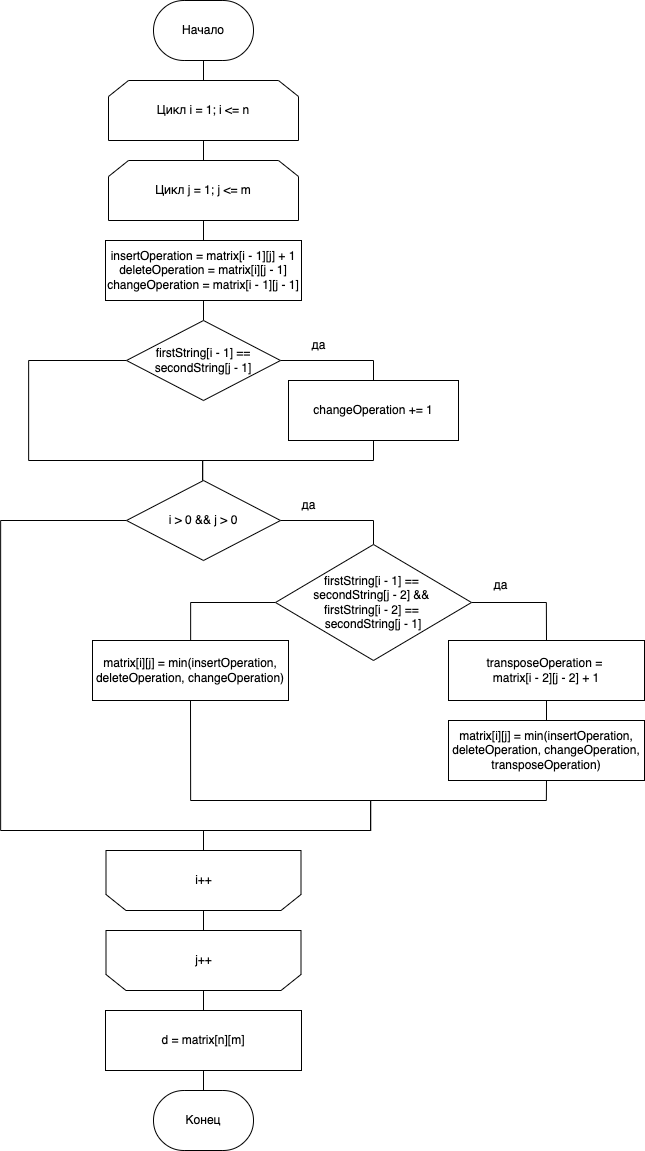
\includegraphics[scale=0.6]{img/dl_iter.png}}
		
	\caption{Схема алгоритма поиска расстояния Дамерау-Левенштейна с заполнением матрицы расстояний}
		
	\label{fig:dl_iter}
\end{figure}


\begin{figure}[h!]
	
	\centering{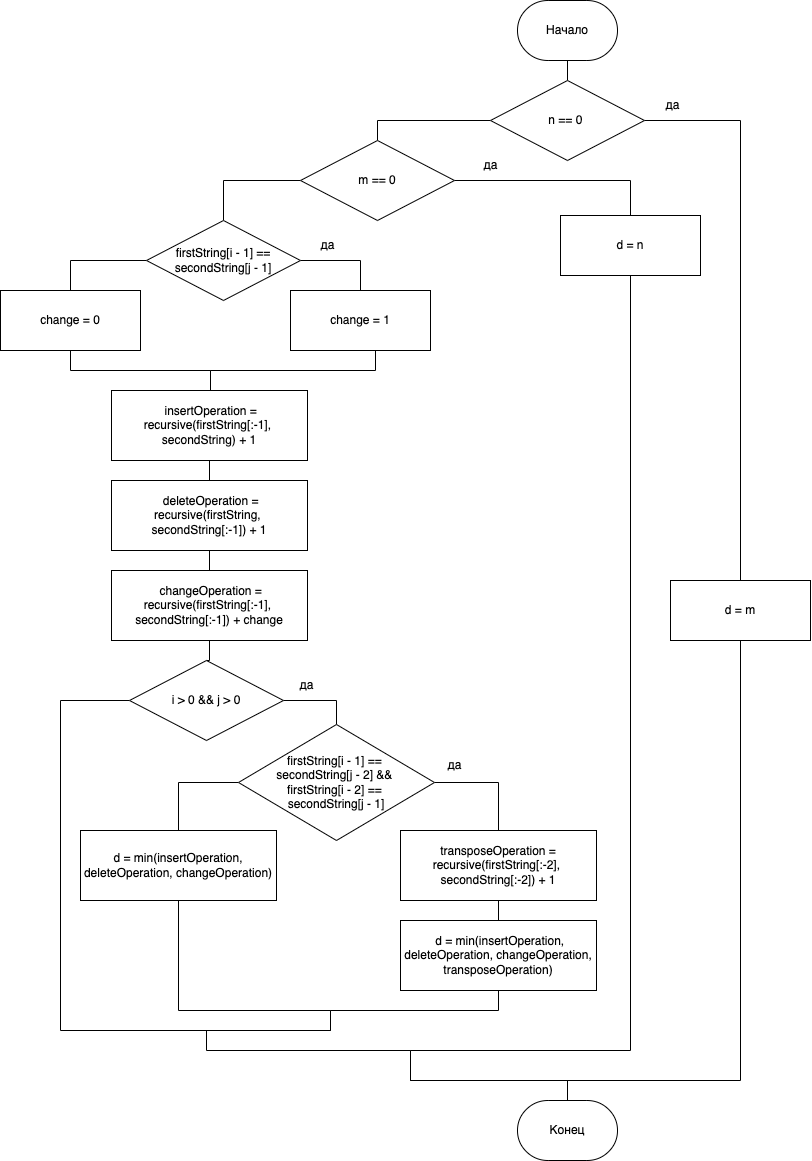
\includegraphics[scale=0.6]{img/dl_recursive.png}}
		
	\caption{Схема рекурсивного алгоритма поиска расстояния Дамерау-Левенштейна без кэширования}
		
	\label{fig:dl_recursive}
		
\end{figure}

\begin{figure}[h!]
	
	\centering{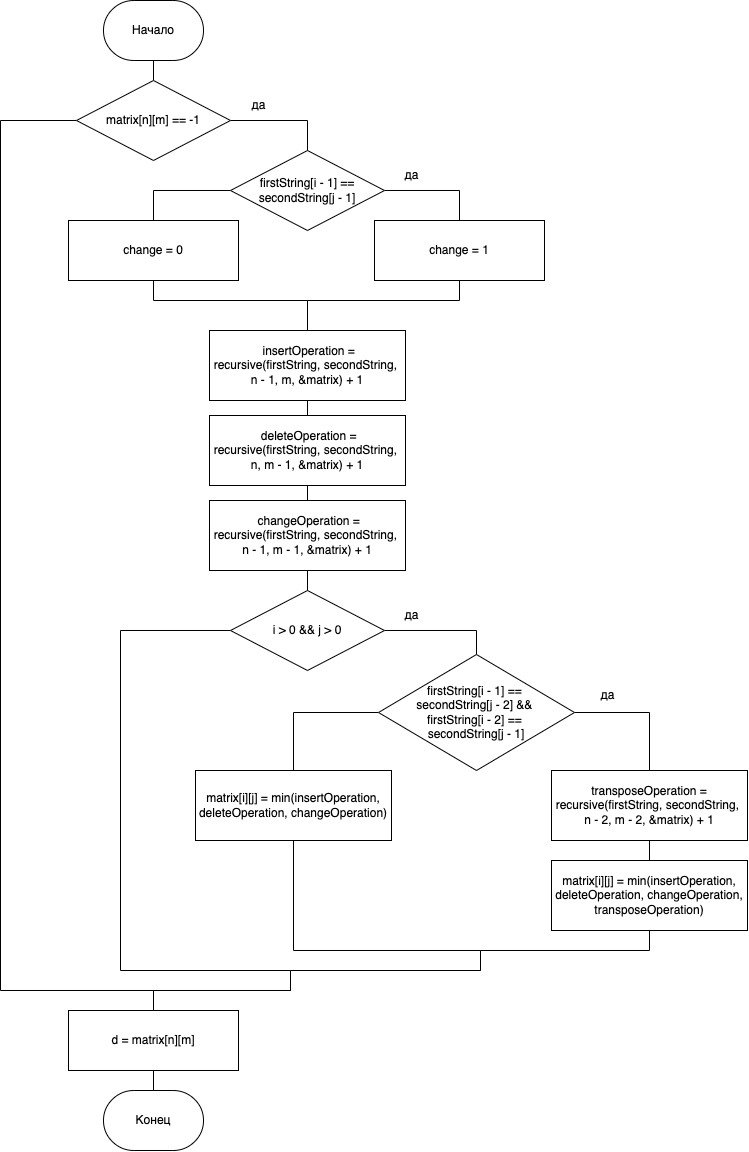
\includegraphics[scale=0.6]{img/dl_cash.png}}
		
	\caption{Схема рекурсивного алгоритма поиска расстояния Дамерау-Левенштейна с кэшированием}
		
	\label{fig:dl_cash}
		
\end{figure}


\section*{Вывод}

На основе теоретических знаний, полученных в аналитическом разделе, были разработаны схемы алгоритмов, благодаря которым могут быть найдены расстояния Левенштейна и Дамерау-Левенштейна.
